%%%%%%%%%%%%%%%%%%%%%%%%%%%%%%%%%%%%%%%%%%%%%%%%%%%%%%%%%%%%%%%%%%%%%%%%%%%%%%%
\chapter{Описание методов локализации ошибок}\label{analysis}
%%%%%%%%%%%%%%%%%%%%%%%%%%%%%%%%%%%%%%%%%%%%%%%%%%%%%%%%%%%%%%%%%%%%%%%%%%%%%%%
В данном разделе производится обзор методов автоматической редукции. Для каждого подхода приводятся его преимущества и недостатки, а также область применения. Кроме того, рассматриваются существующие в настоящее время системы автоматической редукции программ.

%%%%%%%%%%%%%%%%%%%%%%%%%%%%%%%%%%%%%%%%%%%%%%%%%%%%%%%%%%%%%%%%%%%%%%%%%%%%%%%
\section{Дельта дебаггинг}\label{ddalg}
%%%%%%%%%%%%%%%%%%%%%%%%%%%%%%%%%%%%%%%%%%%%%%%%%%%%%%%%%%%%%%%%%%%%%%%%%%%%%%%
Первые шаги в области автоматической локализации ошибок сделали Зеллер и Хильдебрандт в 2002 году. Они предложили автоматизировать данный процесс для экономии человеческих ресурсов~\cite{zeller2002simplifying}. Подход, который изобрели для этого ученые, называется дельта дебаггинг. Алгоритм представляет собой вариацию двоичного поиска для удаления частей приводящего к отказу программы тестового примера $t$ для создания нового тестового примера $t_{min}$, удовлетворяющего двум условиям:
\begin{itemize}
\item $t_{min}$ также приводит к отказу программы;
\item при удалении какой-либо части из $t_{min}$ получается тестовый пример, не приводящий к сбою.
\end{itemize}
Далее приведено описание алгоритма дельта дебаггинга (ddmin).

Пусть даны $test$ и $c_x$, такие что $test(c_x)$ приводит к сбою программы. Необходимо найти $c'_x = ddmin(c_x)$, такое что $c'_x \subseteq c_x, test(c'_x) = fail$. Чтобы найти минимальную тестовую выборку, невозможно просто пытаться удалить каждый элемент по очереди. Поэтому в алгоритме используется бинарный поиск: исходная тестовая выборка делится на 2 равные части $\Delta_1$ и $\Delta_2$ и производится запуск теста на каждой из них. Возможны следующие варианты:
%
\begin{itemize}
\item происходит сбой на подвыборке $\Delta_1$;
\item на подвыборке $\Delta_1$ программа отрабатывает корректно, но на подвыборке $\Delta_2$ происходит сбой;
\item ни одна из подвыборок не приводит к сбою.
\end{itemize}
%
В первых двух случаях мы можем продолжить искать минимальную тестовую выборку в подвыборке, которая привела к сбою. Предположим, что к программному сбою приводит последний элемент тестового примера. Процесс редукции для этого случая показан в таблице~\ref{tab:ddminex}. Минимальная тестовая выборка, приводящая к сбою программы, была найдена на 5 шаге.
%
\begin{table}[]
\center
\captionsetup{skip=5pt}
\caption{\label{tab:ddminex}Пример работы алгоритма дельта дебаггинга}
\begin{tabular}{| c | *{4}{c} | c |}
\hline
\bf Шаг & \multicolumn{4}{|c|}{\bf Выборка} & {\bf Итог}\\
\hline
1 &  1 & 2 & 3 & 4 & fail \\
\hline
2 &  1 & 2 & . & . & ok \\
\hline
3 &  . & . & 3 & 4 & fail \\
\hline
4 &  . & . & 3 & . & ok \\
\hline
5 &  . & . & . & 4 & fail \\
\hline
\end{tabular}
\end{table}

Теперь рассмотрим вариант, когда ни одна из подвыборок не приводит к сбою. В этом случае применяется разбиение выборки на б\'{о}льшее число подмножеств $\Delta_i$, также формируется вся остальная выборка без данного подмножества: $\nabla_i = c_x - \Delta_i$. Пусть производится деление тестовой выборки $c_x$ на $n$ частей. Параметр $n$ называется гранулированностью выборки. Далее необходимо протестировать программу на подвыборках $\Delta_0,...,\Delta_n$, а затем на $\nabla_0,...,\nabla_n$. Возможны следующие варианты:
%
\begin{itemize}
\item происходит сбой на подвыборке $\Delta_i$ --- принимаем $\Delta_i$ как новую тестовую выборку и продолжаем работать с ней, начиная с $n = 2$;
\item происходит сбой на подвыборке $\nabla_i$ --- принимаем $\nabla_i$ как новую тестовую выборку и продолжаем работать с ней, начиная с $n = n - 1$. Гранулированность принимает такую величину для избегания лишней работы, так как большое количество подвыборок с меньшей гранулированностью уже было протестировано;
\item если никакая из подвыборок не приводит к сбою, увеличиваем гранулированность и принимаем $n = 2n$. Это производится только тогда, когда~$2n > |c_x|$, в противном случае алгоритм заканчивает свою работу.
\end{itemize}
%
Обобщенный алгоритм дельта дебаггинга приведен на рисунке~\ref{ddminalg}.
%
\begin{figure}[H]
	$ddmin(c_x) = ddmin_2(c_x, 2)$ где \\
\[ ddmin_2(c'_x, n) =
  \begin{cases}
    ddmin_2(\Delta_i, 2)       & \quad \text{если } test(\Delta_i) = fail\\
    ddmin_2(\nabla_i, max(n - 1, 2))       & \quad \text{если } test(\nabla_i) = fail\\
    ddmin_2(c'_x, min(|c'_x|, 2n))       & \quad \text{если } n < |c'_x|\\
    c'_x & \quad \text{в противном случае}
  \end{cases}
\]
\\
где $\nabla_i = c'_x - \Delta_i, c'_x = \Delta_1 \cup \Delta_2 \cup ... \cup \Delta_n$, все $\Delta_i$ попарно не пересекаются
\caption{Алгоритм дельта дебаггинга}
\label{ddminalg}
\end{figure}
%
В таблице~\ref{tab:ddminex2} приведен пример работы алгоритма дельта дебаггинга. В качестве тестируемого объекта используется программа, в которой происходит сбой, если подать на вход подряд два одинаковых числа.
%
\begin{table}[H]
\center
\captionsetup{skip=5pt}
\caption{\label{tab:ddminex2}Пример работы алгоритма дельта дебаггинга}
\small
\begin{tabular}{| c | *{8}{c} | c | c |}
\hline
\bf Шаг & \multicolumn{8}{|c|}{\bf Выборка} & {\bf Итог} & {\bf Комментарий}\\
\hline
1 &  8 & 3 & 1 & 5 & 7 & 4 & 4 & 1  & fail & \\
\hline
2 &  8 & 3 & 1 & 5 & . & . & . & .  & ok & \\
\hline
3 &  . & . & . & . & 7 & 4 & 4 & 1 & fail & новая подвыборка\\
\hline
4 &  . & . & . & . & 7 & 4 & . & . & ok & \\
\hline
5 &  . & . & . & . & . & . & 4 & 1 & ok & $n = 2n$\\
\hline
6 &  . & . & . & . & 7 & . & . & . & ok & \\
\hline
7 &  . & . & . & . & . & 4 & . & . & ok &\\
\hline
8 &  . & . & . & . & . & . & 4 & . & ok &\\
\hline
9 &  . & . & . & . & . & . & . & 1 & ok &тестируем $\nabla_i$\\
\hline
10 &  . & . & . & . & . & 4 & 4 & 1 & fail &новая подвыборка\\
\hline
11 &  . & . & . & . & . & 4 & 4 & . & fail &новая подвыборка\\
\hline
12 &  . & . & . & . & . & 4 & . & . & ok &\\
\hline
13 &  . & . & . & . & . & . & 4 & . & ok & конец\\
\hline
\end{tabular}
\end{table}
%
Как видно из примера, дельта дебаггинг успешно редуцирует вход программы до минимального, на котором происходит ошибка. Главным недостатком дельта дебаггинга является то, что он не учитывает структурированность ввода и поэтому слабо подходит для редукции сложных данных.

%%%%%%%%%%%%%%%%%%%%%%%%%%%%%%%%%%%%%%%%%%%%%%%%%%%%%%%%%%%%%%%%%%%%%%%%%%%%%%%
\subsection{Дельта дебаггинг с использованием \texttt{topformflat}}
%%%%%%%%%%%%%%%%%%%%%%%%%%%%%%%%%%%%%%%%%%%%%%%%%%%%%%%%%%%%%%%%%%%%%%%%%%%%%%%
Ученые МакПик и Уилкерсон реализовали алгоритм дельта дебаггинга~\cite{delta} для языка C, в котором учли возможную структурированность входного теста. Для этого они использовали утилиту \texttt{topformflat}, которая описана далее.

Примером структурированного входного теста является текст программы. Предположим, что производится тестирование компилятора и при этом происходит сбой на каком-то тестовом примере, который и необходимо минимизировать. Для этого исходный код представляется как множество строк, и алгоритм дельта дебаггинга будет работать на уровне строк. Для учета структурированности как раз и используется \texttt{topformflat} --- простая утилита для обработки вложенности в языке программирования~C. 

Глубина вложенности строки исходного кода --- количество блоков, в которых находится эта строка. На рисунке~\ref{img:topformflatex} приведен пример кода и глубина вложенности каждой строки.
%
\begin{figure}
\center
\begin{tabular}{ |c|c|c| } 
\hline
\bf Код & \bf Глубина  \\
\hline
\tt
\multirow{7}{18em}{int gcd (int a, int b) \{ \\
\ \ \ \ if (b == 0) \{ \\
\ \ \ \ \ \ \ \ return a; \\
\ \ \ \ \} else \{ \\
\ \ \ \ \ \ \ \ return gcd (b, a \% b); \\
\ \ \ \ \} \\
\}
} & 0\\ 
& 1 \\ 
& 2  \\ 
& 1 \\ 
& 2  \\ 
& 1 \\ 
& 0 \\
\hline
\end{tabular}
\caption{\label{img:topformflatex}Пример кода на языке С с указанием вложенности строк}
\end{figure}
%
На вход утилите подается желаемая глубина и текст программы. На выходе получается программа с глубиной вложенности не более заданной. Это происходит путем удаления переводов строк и конкатенации строк с глубиной, более заданной, с предыдущей строкой. На рисунке~\ref{img:topformflatex1} приведен пример применения утилиты с глубиной 1.
%
\begin{figure}
\center
\begin{tabular}{ |c|c|c| } 
\hline
\bf Код & \bf Глубина  \\
\hline
\tt
\multirow{4}{18em}{int gcd (int a, int b) \{ \\
\ \ \ \ if (b == 0) \{ return a; \} \\
\ \ \ \ else \{ return gcd (b, a \% b); \} \\
\}
} & 0\\ 
& 1 \\ 
& 1  \\ 
& 0 \\
\hline
\end{tabular}
\caption{\label{img:topformflatex1}Пример применения утилиты topformflat}
\end{figure}

Утилита topformflat легко интегрируется в алгоритм дельта дебаггинга. Суть использования данной утилиты состоит в том, что нужно применять алгоритм дельта дебаггинга, постепенно увеличивая глубину вложенности исходного кода, начиная с нулевой. Несмотря на то, что данный алгоритм позволяет существенно снизить количество синтаксически некорректных тестов, главный его недостаток заключается в том, что глубина вложенности рассчитывается по фигурным скобкам, поэтому она применима к ограниченному количеству языков программирования в ограниченном количестве случаев. Еще одним недостатком данного метода является то, что он работает на уровне строк, поэтому удалять из программы будут только строки, что недостаточно для качественной редукции.

%%%%%%%%%%%%%%%%%%%%%%%%%%%%%%%%%%%%%%%%%%%%%%%%%%%%%%%%%%%%%%%%%%%%%%%%%%%%%%%
\subsection{Иерархический дельта дебаггинг}\label{hddalg}
%%%%%%%%%%%%%%%%%%%%%%%%%%%%%%%%%%%%%%%%%%%%%%%%%%%%%%%%%%%%%%%%%%%%%%%%%%%%%%%
В 2006 году ученые Мишерги и Су решили проблему применения алгоритма дельта дебаггинга к иерархическим структурам данных~\cite{misherghi2006hdd}, применяя данный алгоритм к дереву разбора, представляющему входной тест. Дельта дебаггинг применяется поочередно, начиная с верхнего, к каждому уровню синтаксического дерева. Полученный алгоритм \emph{иерархического} дельта дебаггинга представлен на рисунке~\ref{alg:hdd}. Сначала задается уровень, с которого начинается обработка дерева. Далее собираются все узлы дерева заданной глубины, для этого используется обход в ширину. Если на текущем уровне дерева есть узлы, то для них применяется процедура дельта дебаггинга, которая находит минимальную конфигурацию узлов данного уровня, на которой происходит сбой программы. После этого из дерева удаляются все нерелевантные узлы и производится переход на следующий уровень.


\begin{figure}[h]
\textbf{ВХОД:} $tree$ --- синтаксическое дерево, представляющее редуцируемую программу \\
\textbf{ВЫХОД:} $tree$ --- редуцированное синтаксическое дерево \\
\begin{algorithmic}[1]
\STATE $level \Leftarrow 0$
\STATE $nodes \Leftarrow \text{getNodes}(tree, level)$
\WHILE{$nodes != 0$} 
	\STATE $min \Leftarrow \text{DDMIN}(nodes)$
	\STATE $\text{removeNodes}(tree, level, minconfig)$
	\STATE $level \Leftarrow level + 1$
	\STATE $nodes \Leftarrow \text{getNodes}(tree, level)$
\ENDWHILE
\end{algorithmic}
\caption{Алгоритм иерархического дельта дебаггинга}
\label{alg:hdd}
\end{figure}

 
Рассмотрим пример работы алгоритма. Пусть производится тестирование компилятора и происходит сбой при компиляции кода, приведенного на рисунке~\ref{ex1:hdd} из-за оператора декремента~\texttt{b} в блоке~\texttt{while}. На рисунке~\ref{ex:hdd} представлен результат применения алгоритма иерархического дельта дебаггинга к синтаксическому дереву, представляющему код, приведенный на рисунке~\ref{ex1:hdd}. Минимизированное дерево соответствует коду, приведенному на рисунке~\ref{ex2:hdd}
%
\begin{figure}
\begin{lstlisting}
fun f() {
    val a = 1
    var b = 0
    if (a != 0) {
        b += 1
    } else {
        b += 2
    }
    while (b != 0) {
        --b
    }
}
\end{lstlisting}
\caption{\label{ex1:hdd}Код, гипотетически приводящий к ошибке компилятора}
\end{figure}

\begin{figure}[h]
\begin{subfigure}[t]{\linewidth}
\center{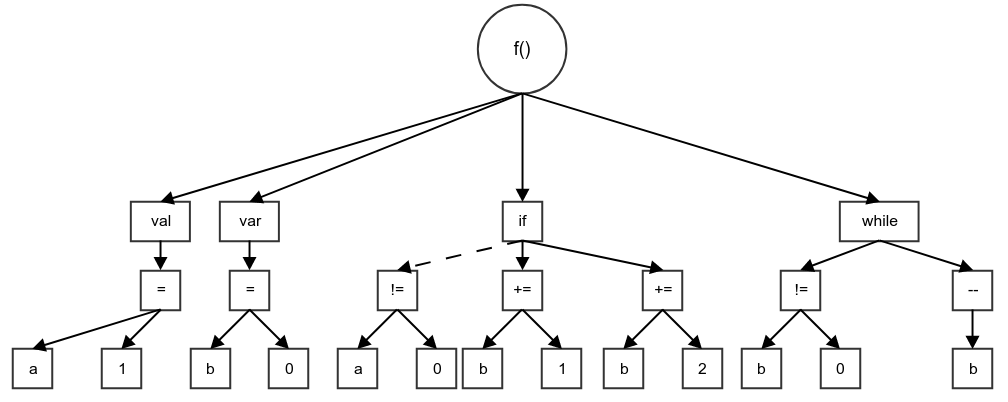
\includegraphics[width=0.99\linewidth]{fig/hddexample}}
\caption{Синтаксическое дерево до редукции}
\end{subfigure}
\begin{subfigure}[t]{\linewidth}
\center{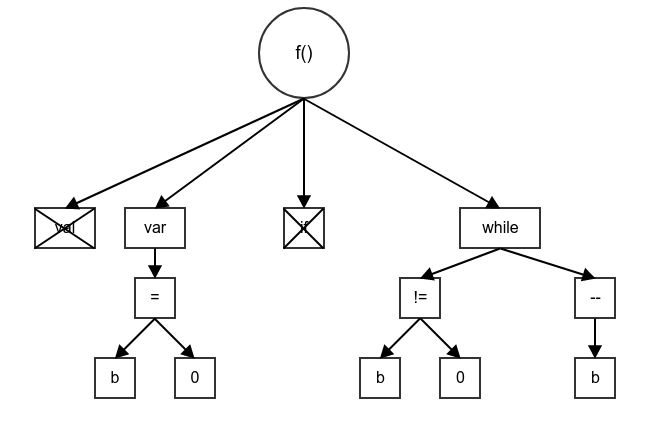
\includegraphics[height=0.3\textheight]{fig/hddexample2}}
\caption{Результат применения алгоритма}
\end{subfigure}
\caption{Пример работы алгоритма иерархического дельта дебаггинга}
\label{ex:hdd}
\end{figure}

\begin{figure}
\begin{lstlisting}
fun f() {
    var b = 0
    while (b != 0) {
        --b
    }
}
\end{lstlisting}
\caption{\label{ex2:hdd}Результат работы алгоритма иерархического дельта дебаггинга}
\end{figure}

Преимуществом данного алгоритма является его применимость к любому виду входных тестовых примеров и лучшие по сравнению с классическим дельта дебаггингом результаты работы. Недостатками являются необходимость построения дерева, скорость работы и невозможность удаления связанных элементов синтаксического дерева, находящихся на разных уровнях.

%%%%%%%%%%%%%%%%%%%%%%%%%%%%%%%%%%%%%%%%%%%%%%%%%%%%%%%%%%%%%%%%%%%%%%%%%%%%%%%
\section{Программные срезы}\label{slicing}
%%%%%%%%%%%%%%%%%%%%%%%%%%%%%%%%%%%%%%%%%%%%%%%%%%%%%%%%%%%%%%%%%%%%%%%%%%%%%%%
Вайзером в работе~\cite{weiser1981program} вводится понятие slicing~(слайсинг)~--- выделение из программы ее определенных частей, называемыми программными срезами. Срез программы определяется по критерию, который, как правило, определяется парой \textit{(точка программы, множество переменных)}. Для заданного критерия срез программы должен содержать только те элементы программы, которые прямым или косвенным образом влияют на переменные из критерия. Задача вычисления срезов получила название слайсинг~\cite{2002slicing}. На рисунке~\ref{ex:slice} приведен пример программы и ее среза относительно критерия \textit{(12, \{TOTAL\})},  где первый элемент критерия --- точка программы, а второй --- переменная.
%
\begin{figure}[]
\centering
\begin{subfigure}[t]{\linewidth}
\begin{lstlisting}[style = pascal]
BEGIN
READ(X,Y)
TOTAL := 0.0
SUM := 0.0
IF X <= 1
	THEN SUM := Y
	ELSE BEGIN
		READ(Z)
		TOTAL := X*Y
		END
WRITE(TOTAL, SUM)
END.
\end{lstlisting}
\caption{Исходный код}
\end{subfigure}
\begin{subfigure}[t]{\linewidth}
\begin{lstlisting}[style = pascal]
BEGIN
READ(X,Y)
TOTAL := 0.0
IF X <= 1
	THEN 
	ELSE TOTAL := X*Y
END.
\end{lstlisting}
\caption{Срез относительно критерия \textit{(12, \{TOTAL\})}}
\end{subfigure}

\caption{Пример программного среза}
\label{ex:slice}
\end{figure}
%
В подходе~\cite{weiser1981program} слайсинг выполняется в соответствии с имеющимися зависимостями по данным и по управлению. Для вычисления срезов используется только статическая информация. 

Ученые Оттенштейны~\cite{ottenstein1984program} предложили еще один подход, который состоял в разрешении проблемы достижимости в графе программных зависимостей (ГПЗ). ГПЗ --- это ориентированный граф, где вершинами являются операторы и выражения программы, а дугами --- зависимости по управлению и по данным между ними. Срез соответствует всем вершинам графа, из которых достижима вершина из критерия.

Все перечисленные срезы вычисляются при обратном проходе графа и используют только статическую информацию.
Полученные таким образом срезы называются обратными статическими срезами. Бергеретти и Карре~\cite{bergeretti1985information} впервые определили понятие прямых статических срезов. Прямой срез состоит из всех операторов и выражений, зависящих от критерия. Оператор зависит от критерия среза, если значения, вычисленные в этом операторе, зависят от значений, вычисленных по критерию среза, или если значения, вычисленные по критерию среза, определяют, будет ли исполняться рассматриваемый оператор или нет~\cite{tip1994survey}. Обратный и прямой срезы вычисляются аналогичным образом; последний требует отслеживания зависимостей в прямом направлении.

Помимо статических существуют и динамические срезы. Отличие состоит в том, что в случае динамического среза рассматриваются только те зависимости между элементами программы, которые возникают при ее конкретном исполнении. В отличие от критерия статического среза, критерий динамического задается тройкой \textit{(входные данные, вхождение оператора, множество переменных)}. На рисунке~\ref{ex:dynslice} приведен пример программы и ее динамического среза относительно критерия \textit{(2, 7, \{TOTAL\})}. Первый элемент критерия~--- входные данные (в случае с примером, значение переменной $x$), второй элемент~--- точка программы, а третий~--- переменная.
%
\begin{figure}[]
\centering
\begin{subfigure}[t]{\linewidth}
\begin{lstlisting}[style = pascal]
BEGIN
READ(X)
TOTAL := 0.0
IF X <= 1
	THEN TOTAL := X + 1
	ELSE TOTAL := TOTAL + X
WRITE(TOTAL)
END.
\end{lstlisting}
\caption{Исходный код}
\end{subfigure}
\begin{subfigure}[t]{\linewidth}
\begin{lstlisting}[style = pascal]
BEGIN
READ(X)
TOTAL := 0.0
IF X <= 1
	THEN
	ELSE TOTAL := TOTAL + X
WRITE(TOTAL)
END.
\end{lstlisting}
\caption{Срез относительно критерия \textit{(2, 7, \{TOTAL\})}}
\end{subfigure}
\caption{Пример динамического программного среза}
\label{ex:dynslice}
\end{figure}

Преимуществами слайсинга являются точность и скорость работы. Главным недостатком является сложность реализации, поскольку для современных языков программирования, использующих динамическую память, необходимо реализовать анализ указателей~\cite{deutsch1994interprocedural}, который позволяет определить, могут ли два указателя ссылаться на один и тот же участок памяти. В дополнение к этому необходимо учитывать все уровни абстракции для языков, реализующих объектно-ориентированную методологию.

%%%%%%%%%%%%%%%%%%%%%%%%%%%%%%%%%%%%%%%%%%%%%%%%%%%%%%%%%%%%%%%%%%%%%%%%%%%%%%%
\section{Существующие средства программной редукции}
%%%%%%%%%%%%%%%%%%%%%%%%%%%%%%%%%%%%%%%%%%%%%%%%%%%%%%%%%%%%%%%%%%%%%%%%%%%%%%%
Существует несколько инструментов для редукции программного кода. Первый из них называется Picireny и описывается в статье~\cite{hodovan2017tree}. Picireny --- реализация алгоритма иерархического дельта дебаггинга. Данный фреймворк является универсальным, принимает на вход грамматику, с помощью ANTLR~\cite{parr2013definitive} строит дерево разбора, над которым и производятся все манипуляции. Преимущества и недостатки у фреймворка те же, что и у алгоритма иерархического дельта дебаггинга, которые были перечислены ранее. 

В настоящее время существует несколько инструментов программного среза для языков программирования Java~\cite{gosling2000java} и C\texttt{++}~\cite{ellis1990annotated}: JSlice~\cite{WR:04}, Indus~\cite{jayaraman2005kaveri}, JavaBST~\cite{abdallah2017javabst} и CodeSurfer~\cite{anderson2004codesurfer}. Данные инструменты реализуют различные по сложности и качеству работы алгоритмы слайсинга. Стоит отметить, что методы программного среза и дельта дебаггинга не являются взаимоисключающими, --- их можно использовать вместе, например, перед дельта дебаггингом запустить быстрый статический слайсинг, который значительно упростит целевой тестовый пример.

Наиболее развитым в данный момент инструментом редукции программ можно смело назвать Creduce~\cite{regehr2012test}. Creduce разработан для редукции тестовых примеров для компиляторов языков С/C\texttt{++}, в частности --- результатов работы генератора случайных тестов Csmith~\cite{yang2011finding}, которые (будучи случайно сгенерированными) обычно содержат огромное количество нерелевантной ошибке информации. Creduce является гибридным средством, состоящим из следующего набора трансформаций:
%
\begin{itemize}
	\item дельта дебаггинг с использованием topformflat;
	\item более тридцати трансформаций над исходным кодом, например: встраивание небольших функций, удаление неиспользуемых функций и переменных, удаление неиспользуемого аргумента из функции и т.д.;
	\item форматирование получившегося кода.
\end{itemize}
%
Результаты тестирования данного средства показали его успешность при решении поставленных задач~\cite{groce2016cause}. Недостатком Creduce является то, что он работает только с языками программирования~C/C\texttt{++}.

%%%%%%%%%%%%%%%%%%%%%%%%%%%%%%%%%%%%%%%%%%%%%%%%%%%%%%%%%%%%%%%%%%%%%%%%%%%%%%%
\section{Резюме}
%%%%%%%%%%%%%%%%%%%%%%%%%%%%%%%%%%%%%%%%%%%%%%%%%%%%%%%%%%%%%%%%%%%%%%%%%%%%%%%
В данном разделе выполнено рассмотрение предметной области локализации программных ошибок. Рассмотрены существующие методики редукции и инструменты, реализующие описанные методики. Подавляющее большинство инструментов предназначены для популярных языков программирования C/C\texttt{++} и Java, поэтому задача создания инструмента редукции для других языков программирования является актуальной.
